\documentclass[border=1mm]{standalone}
% \usepackage[margin=2.5cm]{geometry}

\usepackage{graphicx,tikz,tikz-layers} 
\usetikzlibrary{decorations.markings,calc,positioning,arrows,shapes.geometric,arrows.meta}

\colorlet{myred}{red!80!black}
\colorlet{myblue}{blue!80!black}
\colorlet{mybluee}{myblue!80!black}
\colorlet{mygreen}{green!60!black}
\colorlet{myorange}{orange!70!red!60!black}
\colorlet{mydarkred}{red!20!black}
\colorlet{mydarkblue}{blue!40!black}
\colorlet{mydarkgreen}{green!20!black}


\begin{document}

% \resizebox{\textwidth}{!}{
\tikz[font=\small,scale=1, every node/.style={outer sep=0pt, inner sep=0pt, align=center}, w/.style={minimum width=#1},h/.style={minimum height=#1},s/.style={minimum size=#1}, eu/.style={shorten >=#1},ed/.style={shorten <=#1},line join=round]
{
\tikzset{>={Latex[length=1.5mm, width=1.25mm]}}

\node[] (im) {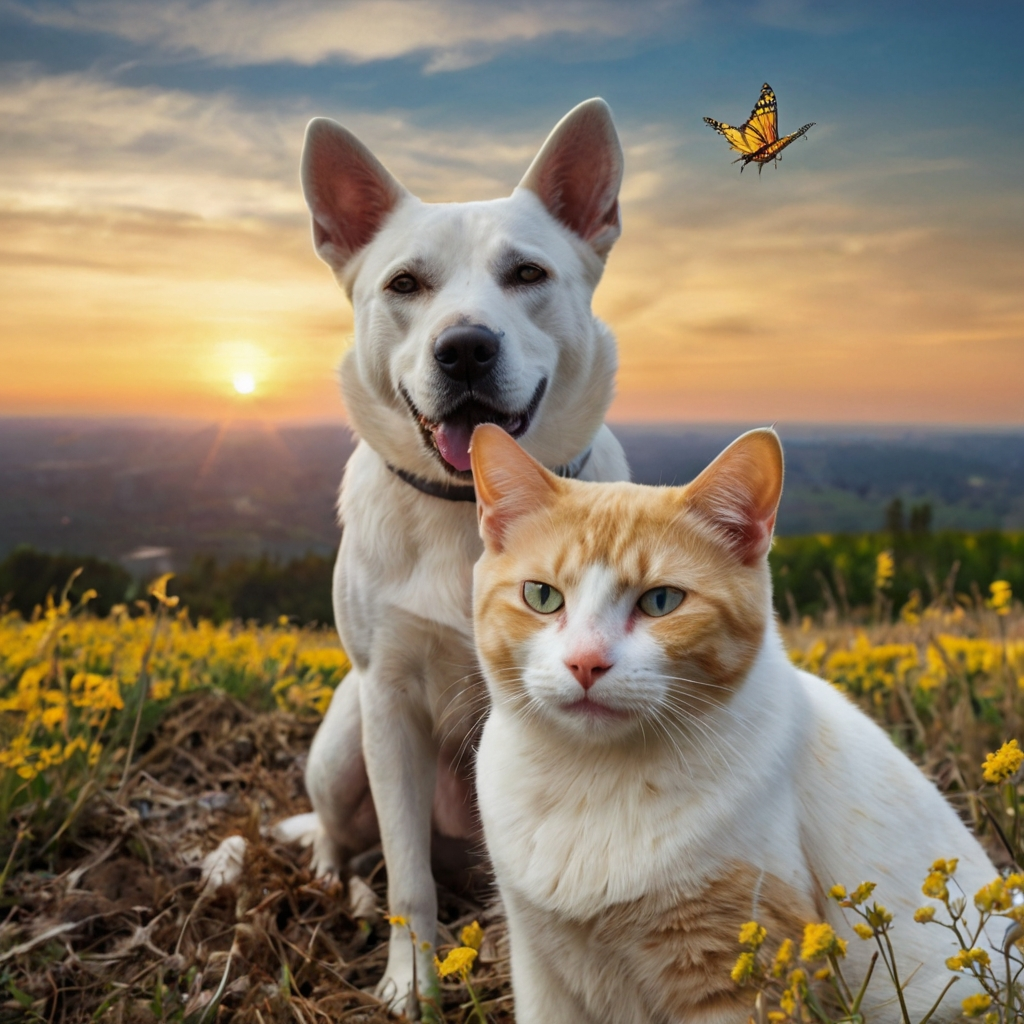
\includegraphics[width=2cm]{images/cat&dog.jpg}};

\node[w=2cm, h=2cm, right=1cm of im] (a) {Backbone\\CNN (VGG)};
\begin{scope}[on behind layer]
 \draw[fill=myblue!15] (a.north west)--(a.south west)--($(a.south east)+(0,.3)$)--($(a.north east)+(0,-.3)$)--cycle;   
\end{scope}

\node[draw, s=2cm, right=1.25cm of a, fill=gray] (b) {};
\draw[fill=gray!35] (b.north west)--($(b.north west)+(-.2,-.2)$)--($(b.south west)+(-.2,-.2)$)--(b.south west)--cycle;
\draw[fill=gray!35] (b.south east)--($(b.south east)+(-.2,-.2)$)--($(b.south west)+(-.2,-.2)$)--(b.south west)--cycle;

\node[draw, s=2cm, right=1.25cm of b, fill=gray] (c) {};
\draw[fill=gray!35] (c.north west)--($(c.north west)+(-.2,-.2)$)--($(c.south west)+(-.2,-.2)$)--(c.south west)--cycle;
\draw[fill=gray!35] (c.south east)--($(c.south east)+(-.2,-.2)$)--($(c.south west)+(-.2,-.2)$)--(c.south west)--cycle;

\node[draw, right=2cm of c, w=1cm, h=2cm, fill=myblue!15]  (d) {\rotatebox{90}{\shortstack{Fully \\ Connected}}};
\node[draw, right=.25cm of d, w=1cm, h=2cm, fill=myblue!15]  (e) {\rotatebox{90}{\shortstack{Fully \\ Connected}}};
\node[draw, right=.75cm of e, w=1cm, h=2cm, yshift=1.1cm, fill=myblue!15]  (f) {\rotatebox{90}{\shortstack{Fully \\ Connected}}};
\node[draw, right=.75cm of e, w=1cm, h=2cm, yshift=-1.1cm, fill=myblue!15]  (g) {\rotatebox{90}{\shortstack{Fully \\ Connected}}};

\node[above=2cm of c] (im1) {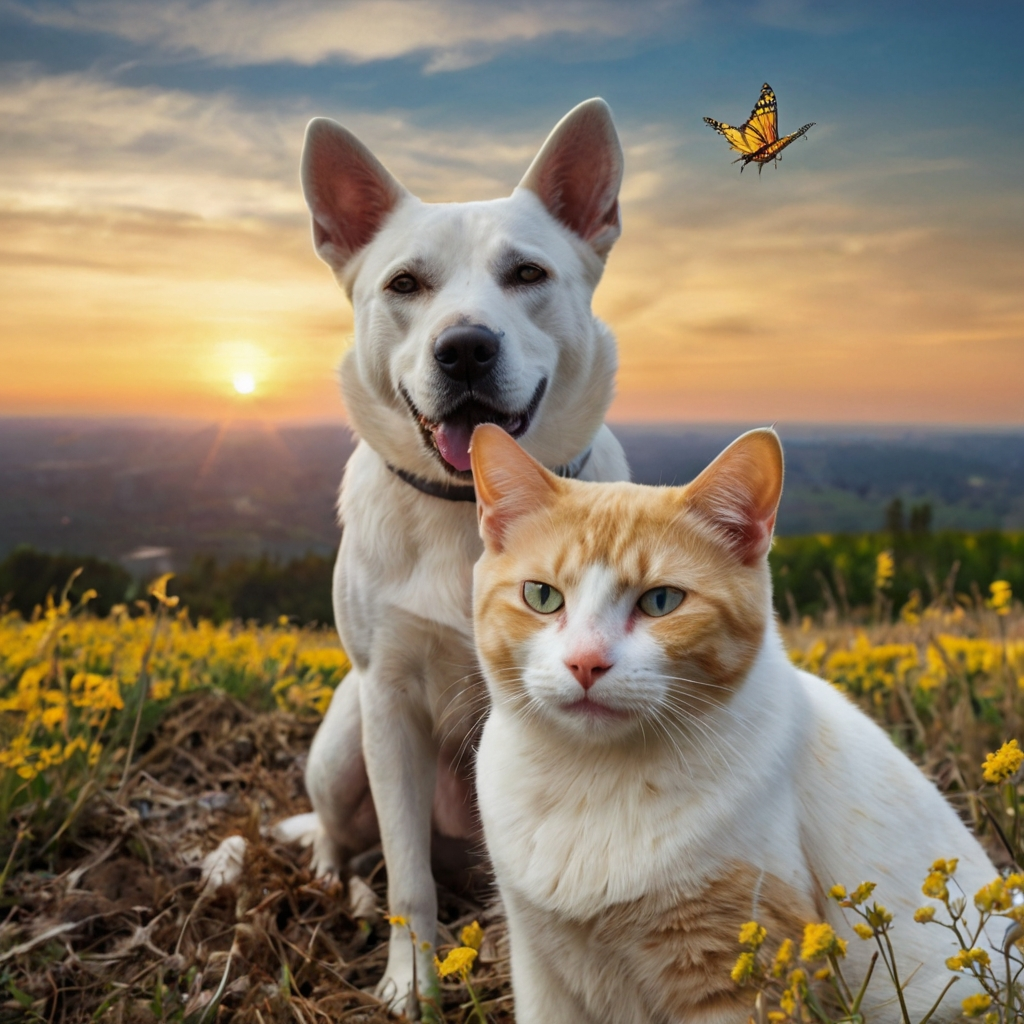
\includegraphics[width=2cm]{images/cat&dog.jpg}};

\node[draw, s=2cm, left=1.25cm of im1, fill=mygreen!15] (h) {Region\\Proposal\\Eg: Selective\\search};

% Arrows
\draw[->] (im)--(a);
\draw[->] (a)--(b);
\draw[] (b)--(c);
\draw[->] (c)--node[above=1.2cm, font=\footnotesize] {ROI pooling Output size\\Op$=[N\times 7\times 7\times 512]$} (d);
\draw[] (d)--(e);
\draw[->] (e.east)--++(.3,0) |- (f);
\draw[->] (e.east)--++(.3,0) |- (g);
\draw[->] (im1)--(c);
\draw[->] (h)--(im1);

% Labels
\node[above=1mm of im] {$1000$};
\node[left=1mm of im] {$600$};

\node[above=1mm of b] {$60$};
\node[right=1mm of b, yshift=4mm] {$40$};
\node[below=3.5mm of b, xshift=4mm] {$512$};

\node[below=3.5mm of c] {ROI Pooling};
\node[right=1mm of im1] {N region proposals};
\node[below=1mm of d] {4096\\units};
\node[below=1mm of e] {4096\\units};
\node[above=1mm of f] {C units};
\node[below=1mm of g] {C$^{4}$ units};
\node[right=4mm of f] {Object\\classification\\Op$=[N\times C]$};
\node[right=4mm of g] {BB\\Regression\\Op$=[N\times C^{4}]$};

\node[draw, red, ultra thick, w=1cm, h=.99cm, anchor=north, xshift=2mm, yshift=2mm] at (im1.center) {};
\node[draw, white, ultra thick, h=1cm, w=.8cm, anchor=south, xshift=-1mm, yshift=-1mm] at (im1.center) {};

\node[draw, red, ultra thick, w=1cm, h=.99cm, anchor=north, xshift=2mm, yshift=2mm] at (c.center) {};
\node[draw, white, ultra thick, h=1cm, w=.8cm, anchor=south, xshift=-1mm, yshift=-1mm] at (c.center) {};

% Orange box
\begin{scope}[on background layer]
\node[draw, dashed, w=17.6cm, h=5.25cm, fill=mybluee!7, anchor=west] (box) at ($(a.west)+(-.5,0)$) {};
\end{scope}

\node[anchor=south, above=2mm] at (box.south) {FAST RCNN Network};
}
% }
\end{document}
